\section{LSST Observing Cadence Optimization to Enhance PHA Completeness \label{sec:opsim}}

The effects of varying the LSST observing strategy on PHA completeness and other science can be evaluated in detail using a combination of the LSST Operations Simulator (OpSim) and the LSST Metrics Analysis Framework (MAF). 

The LSST Operations Simulation (OpSim) is a python software package that generates a realistic pointing history, with the time, filter, location, astronomical conditions, weather conditions, and predicted point-source $5\sigma$ limiting magnitude, for each LSST visit for ten years. This pointing history is generated using weather data (cloudiness and seeing) from the Cerro Pachon site and a high-fidelity model of the telescope itself (including slew and settle time and dome movement, for example), combined with a parameterized set of observing proposals that determine how the scheduling algorithm attempts to gather observations. By configuring OpSim with different parameters for the observing proposals, we can generate a series of simulated surveys which prioritize different science goals. 

The LSST Metrics Analysis Framework (MAF) is a user-oriented, python package for evaluating the pointing history from these simulated surveys in light of particular science goals or interests. The results of metrics coded in the MAF framework can be calculated for any given simulated survey and compared as proposal parameters are changed in OpSim. Metrics will be gathered from as wide a cross section of the astronomical community as possible, together with "figures of merit" that summarize and define 'success' for a given metric. This permits a thorough investigation of the trades between different observing strategies, in terms of the effect on science goals.

We can use MAF to evaluate the effect of various observing strategies on moving object completeness and characterization as well. Here we focus on discovery completeness of Potentially Hazardous Asteroids (PHAs) as both the observing strategy (related to changes in OpSim proposal parameters) and discovery criteria (related to LSST Data Management (DM) and the Moving Object Processing Software (MOPS) workloads) are varied. 

\subsection{Details of MAF analysis}

Using MAF to evaluate metrics for moving objects, such as PHAs, requires first defining the parameters of the input small body population by:

\begin{enumerate}
\item{Defining an orbital distribution for the input moving object population, specified by a set of orbital parameters for each object. Here we have chosen to use an orbital distribution defined by the large ($>1$ km) diameter known PHAs, as reported to the Minor Planet Center (MPC). This population is thought to be relatively complete and thus should be relatively unbiased. For comparison with other completeness estimates which use an Near Earth Object (NEO) population based on the \cite{Bottke2002} model instead of the subset of these objects which are classified as PHAs, we also evaluate completeness using a random sample of 2000 NEOs from the synthetic solar system model presented in \cite{Grav2011}.  A plot of the $a$, $e$, $i$ distribution for these PHAs and NEOs is shown in Figure~\ref{fig:PHA_orbits}.  }
\begin{figure}
\centering
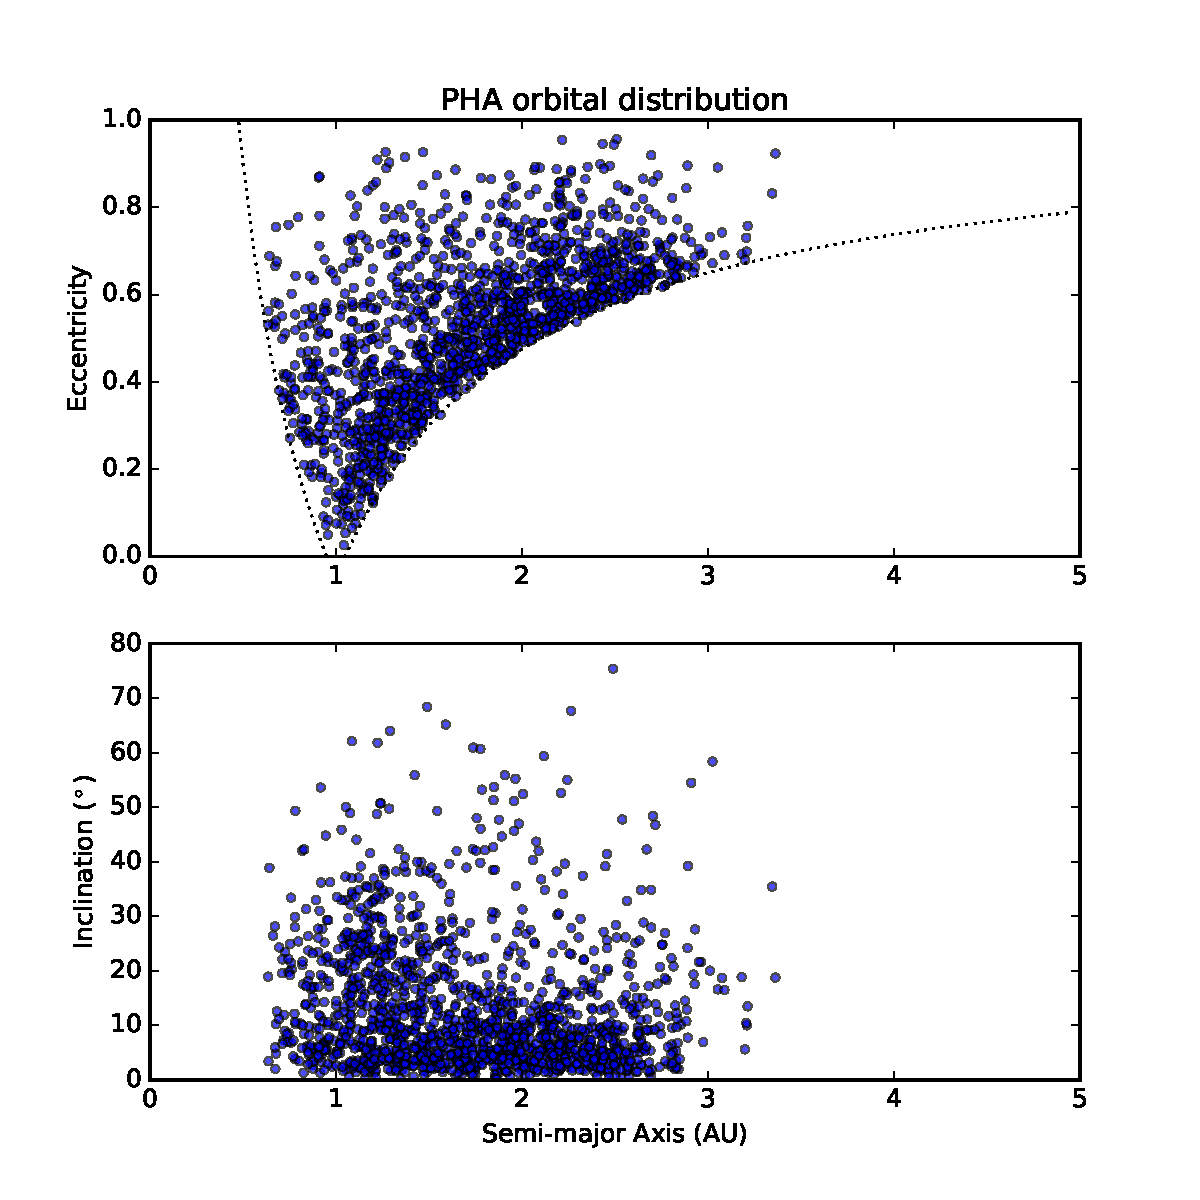
\includegraphics[width=0.45\textwidth]{figures/pha20141031_orbits} 
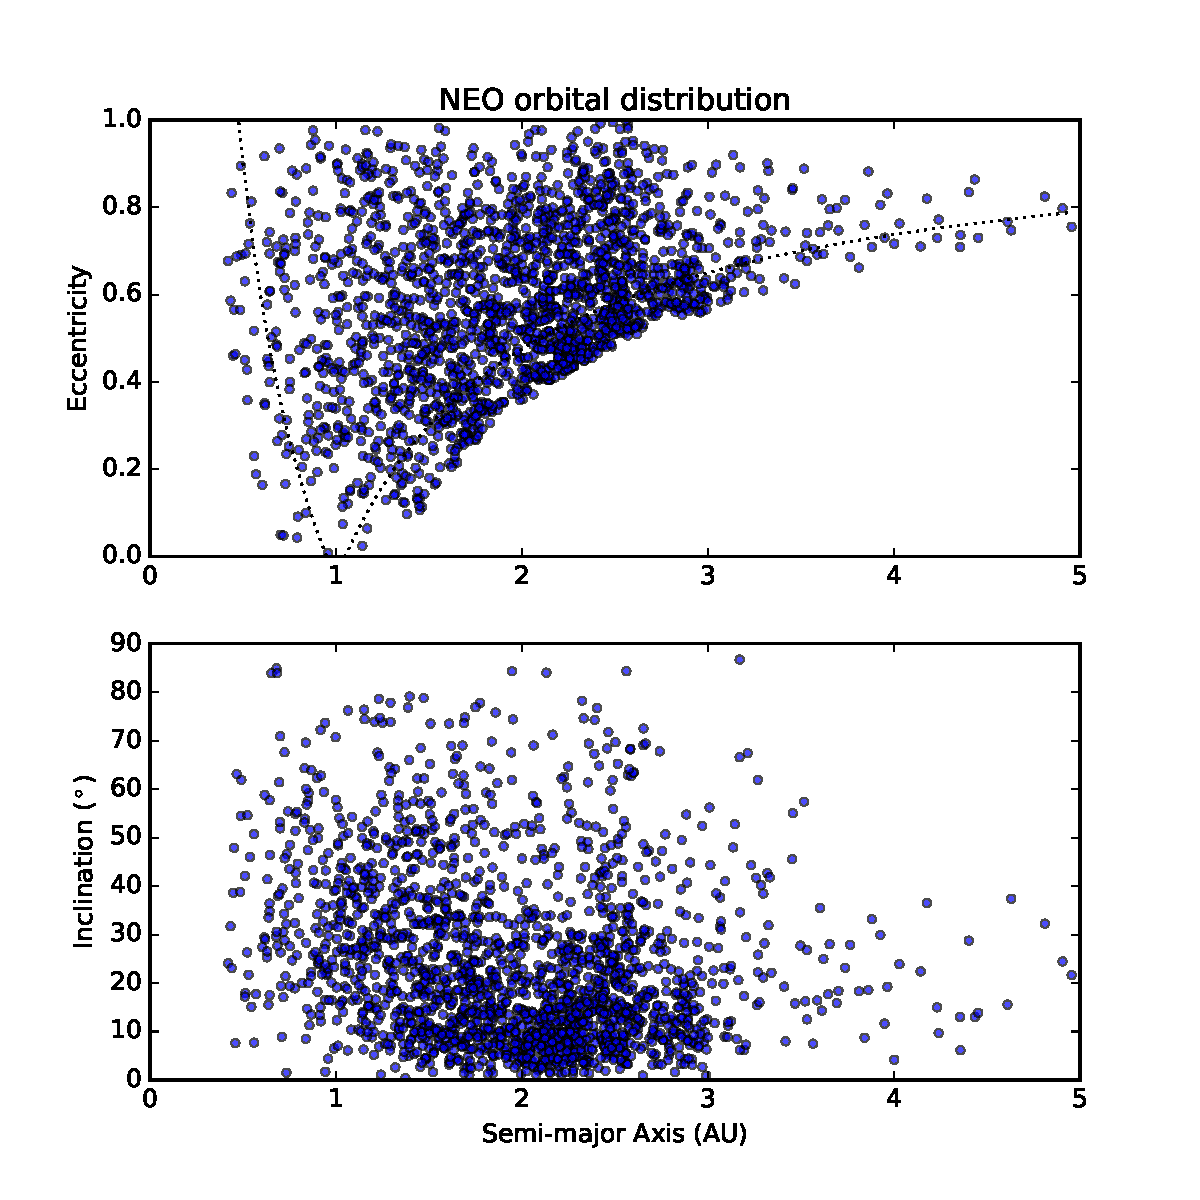
\includegraphics[width=0.45\textwidth]{figures/neos_2k_orbits}
\caption{The eccentricity and inclination distributions, as a function of semi-major axis, of the PHAs (left) and NEOs (right) used in this analysis. The PHA population consists of the orbital distribution of $>1$~km PHAs recorded by the MPC as of 2014 (1511 objects). The NEO population is a random sampling of 2000 NEOs from the S3M \citep{Grav2011}, a synthetic solar system model based on the \cite{Bottke2002} NEO orbital distribution. \label{fig:PHA_orbits}}
\end{figure}

\item{Optionally, define an $H$ magnitude for each object. For populations where the $H$ magnitude distribution is strongly tied to the orbital distribution, this is necessary. However, most small body populations can be well described by independent orbital and $H$ magnitude distributions; the PHA population larger than 140~m in diameter can be generally described in this manner. In these cases, a smaller set of orbits can be used to represent the overall larger population; during analysis, each object can be `cloned' from the fiducial $H$ magnitude associated with the orbit to a range of $H$ magnitudes covering the range interesting for analysis (adjusting the related $m_V$ magnitude). This makes the metric analysis, and particularly the generation of the expected observations for each object, simpler and faster. As long as sufficient resolution of the orbital parameter space is maintained, the metric results over the range of $H$ magnitudes will be comparable to the results calculated with a larger population. Here we use the small population of $>1$~km diameter known PHAs and NEOs, then clone them to a range of $H$ magnitudes between $H$=11 and $H$=28. We have verified with a larger, simulated set of NEOs that reducing the population from 10,000 model NEOs to 2000 model NEOs does not change the calculated survey  completeness. }

\item{Optionally, define a spectrum or color for each object. This facilitates the conversion from $H$ magnitude (assumed to be in $V$ band) to the apparent magnitude in a given LSST observation, which may be in any of $u$, $g$, $r$, $i$, $z$, or $y$ filters. Here we have assumed that our entire PHA population consists of C-type asteroids, with resulting transformations to  LSST bandpasses as described in Table~\ref{tab:sed_colors}.  }

\begin{deluxetable}{ccccccc}
\centering
\tablecolumns{7}
\tablecaption{Color transformations from Harris $V$ band to LSST bandpasses, for C and S type asteroids. \label{tab:sed_colors}}
\tablewidth{0.7\textwidth}
\tablehead{ Type & $V-u$ & $V-g$ & $V-r$ & $V-i$ & $V-z$ & $V-y$  \\ }
\startdata
C  & -1.53 &  -0.28 &  0.18 &  0.29 &  0.30 & 0.30 \\
S & -1.82 &  -0.37 &  0.26 & 0.46 &  0.40 & 0.407  \\
\enddata
\end{deluxetable}

\end{enumerate}

Using the details of the input population, MAF then generates the expected observations of each object using the pointing history from a specific OpSim simulated survey. Ephemerides are generated using OpenOrb \citep{OpenOrb2009} for a closely spaced grid of times, and then interpolated to the exact times of each OpSim pointing. If the object is within the LSST field of view, its predicted position, velocity, and apparent $V$ magnitude (calculated from the fiducial $H$ magnitude associated with the orbit) is recorded along with information about the simulated observation itself (such as the seeing, limiting magnitude, filter, and boresight RA/Dec). The full LSST camera footprint, including chipgaps, is used to determine if an object is within the field of view. The camera footprint is shown in Figure~\ref{fig:camera_footprint}.

\begin{figure}
\centering
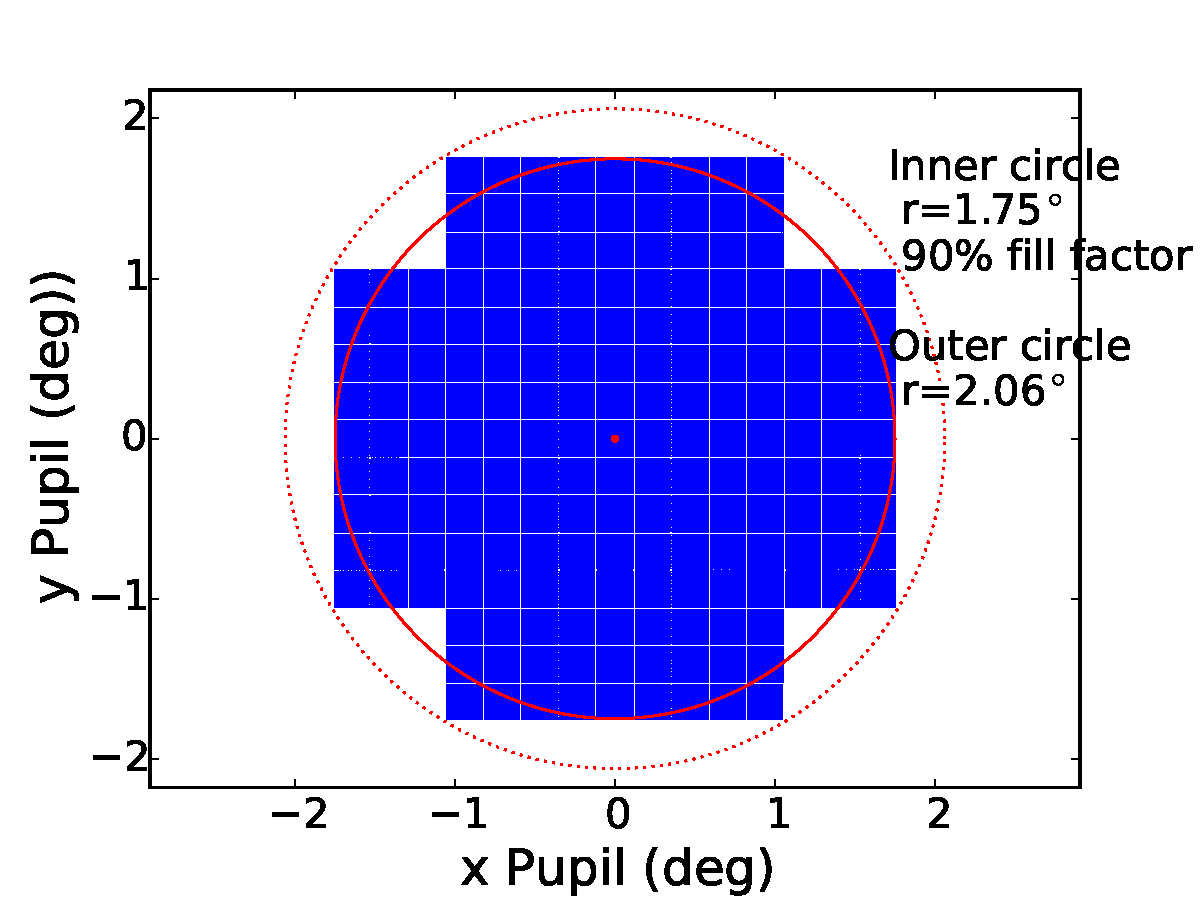
\includegraphics[width=0.65\textwidth]{figures/focalplane} 
\caption{Model of the LSST camera footprint, including chipgaps and CCD + raft layout. \label{fig:camera_footprint}}
\end{figure}

MAF also calculates trailing loss estimates for each observation, which are necessary when evaluating if a particular object is visible in a given observation. Trailing losses occur whenever the movement of an object spreads its photons over a wider area than a simple stellar PSF. There are two aspects of trailing loss to consider: simple SNR losses and detection losses. The first is simply the degradation in SNR that occurs (relative to a stationary PSF) because the trailed object includes a larger number of background pixels in its footprint. This will affect photometry and astrometry, but typically doesn't directly affect whether an object is detected or not. The second effect (detection loss) is not related to measurement errors but does typically affect whether an object passes a detection threshhold. Detection losses occur because source detection software is optimized for detecting point sources; a stellar PSF-like filter is used when identifying sources that pass above the defined threshhold, but this filter is non-optimal for
trailed objects. This can be mitigated with improved software ({\it e.g.} detecting to a lower SNR threshhold and then using a variety of trailed PSF filters to detect sources). Both trailing losses can be fit as:
\begin{eqnarray}
\Delta \, m & = &-1.25 \, log_{10} \left( 1 + \frac{a \, x^2} { 1 + b\,
    x} \right) \\
x & = & \frac{v \, T_{exp}} {24 \, \theta} 
\end{eqnarray}
where $v$ is the velocity (in degrees/day), $T_{exp}$ is the exposure time (in seconds), and $\theta$ is the FWHM (in arcseconds). For SNR trailing losses, we find $a = 0.67$ and $b = 1.16$; for detection losses, we find $a=0.42$ and $b=0$. An illustration of the magnitude of these trailing loss effects for 0.7'' seeing is given in Figure~\ref{fig:trailinglosses}. When considering whether a source would be detected at a given SNR using typical source detection software, the detection loss should be used. With an additional workload on data management, the smaller trailing losses could be used instead.

\begin{figure}
\centering
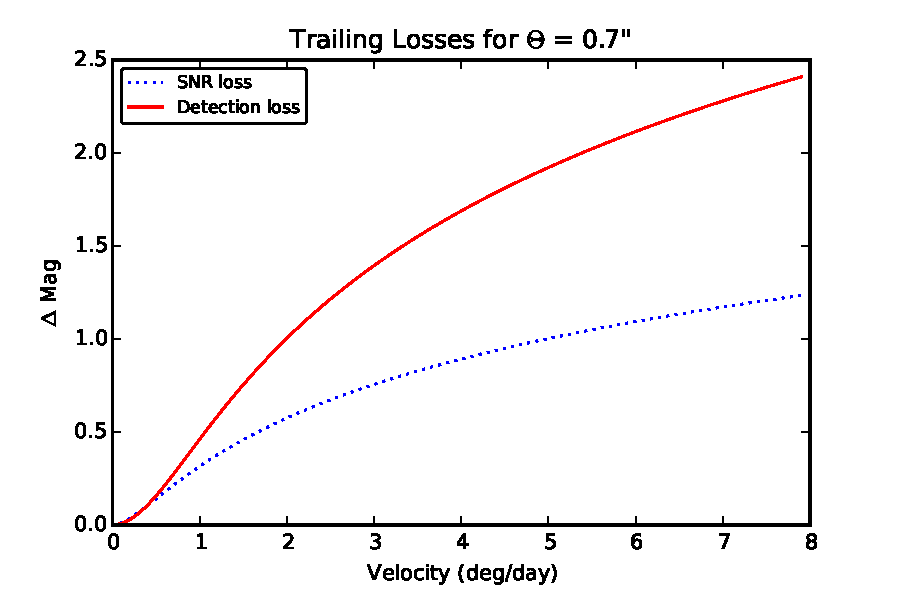
\includegraphics[width=0.5\textwidth]{figures/trailing_losses}
\caption{Trailing losses for 30 second LSST visits, assuming seeing of
  0.7''. The dotted line shows SNR trailing losses, the solid line
  indicates  detection trailing losses. With software improvements
  detection losses can be mitigated.
\label{fig:trailinglosses}}
\end{figure}

From the list of available observations, MAF then evaluates metrics such as the fraction of the input population detected during the survey as a function of $H$ magnitude (equivalent to the differential discovery completeness). This is the core work of MAF -- in general, the list of detections, including 
the $m_V$, trailing losses, color terms and $5\sigma$ limiting magnitude of each detection could be generated by other means (such as the LSST Catalogs Simulation). 

The important metric in the context here is the differential discovery completeness, integrated over the expected $H$ magnitude distribution to find the cumulative discovery completeness. For each object in our small input population, we evaluate the list of observations to see how many sets of these observations meet a given `discovery criteria';  for objects which satisfy the discovery criteria at least once, we count the object as "discovered". This evaluation proceeds as follows:

\begin{enumerate}
\item We are cloning our small input population over a range of $H$ magnitudes, so for each object we must calculate in which visits the object would actually be visible for this discovery criteria - at the current $H$ value being evaluated. We do this assuming appropriate offsets between the $m_V$ recorded in the observation list (calculated assuming the fiducial $H$ magnitude) and the $m_V$ the object would have if it were cloned to the current $H$ value. If a simple SNR cut is desired, the SNR of the resulting apparent magnitude (including color terms and trailing losses) is calculated and the cut applied. If a probabilistic determination of visibility is desired, we calculate the likelihood of detecting this particular source given the $5\sigma$ limiting magnitude and the magnitude of the source and use this to randomly decide if a source was visible in a given visit. The probability of detecting a source is described as:
\begin{eqnarray}
P & = & \frac {1}  {1 +  exp^\frac {m -  m_5}{\sigma}}
\end{eqnarray}
where $m$ is the apparent magnitude of the object (after allowing for color terms and trailing losses),  $m_5$ is the $5\sigma$ limiting magnitude of the visit, and $\sigma$=0.12 describes the width of the falloff \citep{2014ApJ...794..120A}. The basic discovery criteria uses the probabilistic determination of visibility combined with detection losses. We also evaluate more aggressive discovery criteria using trailing losses instead of detection losses, and the most aggressive discovery criteria lowers the visibility requirement to a SNR of 4.

\item Given the set of visits where the object was within the field of view and visible at this $H$ value, we look for visits spaced in time according to the discovery criteria. These criteria generally consist of a given number of visits within a specified time span within a single night, followed by a given number of additional nights (each with the same required number of visits in the same time span) falling within a specified time window. The basic criteria is a pair of visits in each night occurring within 60 minutes, repeated for 3 nights within a 15 day time window. However, we also evaluate the effect of varying the discovery criteria to require triplets or quads of visits within a single night, varying the length of the time window from 15 to 30 days.

\item With each unique set of discovery criteria, we have a record of what objects would be `discovered' at each $H$ value. With this we calculate the differential discovery completeness, the fraction of objects discovered at a given $H$ magnitude. To turn this into a cumulative discovery completeness, we simply integrate over $H$, assuming a given $H$ distribution for the population. We use $dN/dH = 10^{\alpha\, H}$, where $\alpha$ = 0.3.

\end{enumerate}


\subsection{OpSim Simulated Surveys}

The current baseline observing strategy for LSST is represented by our reference run, minion\_1016.  This simulated survey contains observations balanced between several different observing proposals:
\begin{enumerate}
\item The Wide, Fast, Deep (WFD) proposal (also known as the Universal proposal) is the primary LSST survey, expected to receive 85-95\% of the observing time and cover 18,000 square degrees of sky. In the baseline observing strategy, this proposal is configured to obtain visits in pairs spaced about 30 minutes apart, and will typically return to each field about every 3-4 days, balancing the six $ugrizy$ filters. The footprint for the WFD proposal covers approximately 0 to -60 degrees in declination, with a full range of RA values except for a region around the galactic plane. This declination range corresponds to an airmass limit of about 1.3 when the fields are at an Hour Angle of +/- 2 hours. In minion\_1016, the WFD proposal receives 85\% of the total visits.
\item The North Ecliptic Spur (NES) proposal is an extension to the WFD to reach the northern limits of the ecliptic plane (+10 degrees), and allows higher airmass observations. The visit timing is similar to the WFD, although the $u$ and $y$ filter are not requested in this region. In the baseline observing strategy, minion\_1016, each NES field requests about 40\% of the total number of WFD visits per field when considering $griz$ filters only (304 visits per field in $griz$ vs 795 visits per field in $griz$ in WFD), and receives 6\% of the total visits. 
\item The Deep Drilling Fields (DD) proposal includes a set of single pointings that are requested in extended sequences; currently these sequences are $grizy$ visits, with additional coverage in $u$ band. Each sequence requires about an hour of observing time, and is repeated every few days. In minion\_1016, there are 5 DD fields, 4 of which correspond to fields which have been officially selected and announced; these five fields receive 5\% of the total visits. 
\item The Galactic Plane (GP) proposal covers the region around the galactic plane not covered by the WFD, an area where LSST is expected to be highly confused by the density of stellar sources. This proposal requests a small number of visits in each of the six $ugrizy$ filters, with no timing constraints. In minion\_1016, this proposal receives 2\% of the total visits. 
\item The South Celestial Pole (SCP) proposal is an extension of the WFD footprint to cover the region south of -60 degrees declination. Like the GP, this proposal requests a small number of visits in each of the six $ugrizy$ filters, with no timing constraints. In minion\_1016, this proposal receives 2\% of the total visits.
\end{enumerate}. 

The footprint of these various proposals in the baseline minion\_1016 reference run is shown in Figure~\ref{fig:minion_footprints}. In each proposal, the individual visits are 30 seconds long, consisting of two back-to-back coadded 15 second exposures. 

\begin{figure}
\centering
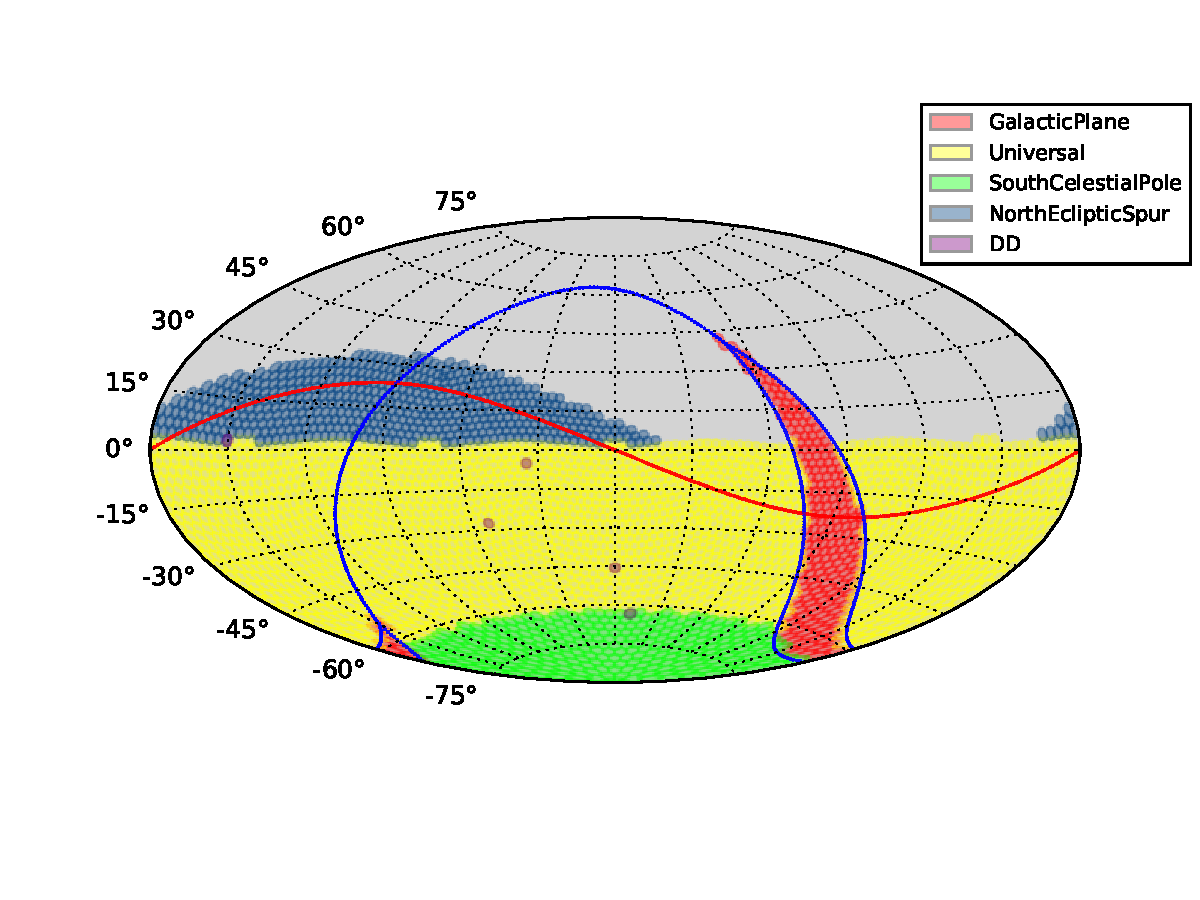
\includegraphics[width=0.5\textwidth]{figures/minion_1016_proposal_footprint}
\caption{The footprints of the various proposals included in the baseline observing strategy, represented by reference run minion\_1016. 
\label{fig:minion_footprints}}
\end{figure}

To investigate the effects of requiring triplets or quads of visits within a single night as part of the discovery criteria, instead of simply pairs, two additional simulated surveys were run where the WFD (but not the NES) requested visits in sequences of three or four, instead of just pairs. It is important to note that due to the behavior of the OpSim software, it is frequently the case that more than the requested minimum number of visits are received in a particular field on a given night. That is, even in the baseline minion\_1016 run, which requested pairs of visits in each night for the WFD and NES, it is often the case that three or four visits were obtained despite the smaller request. Thus, these additional runs provide an indication of the trade-offs in coverage and completeness that result from requesting more visits per field, per night, but the effects would be more pronounced if this behavior of the software did not exist. The simulated surveys enigma\_1281 and enigma\_1282 are the result of requesting triples and quads in the WFD proposal, respectively. 

A series of additional OpSim simulated surveys were created with parameters intended to improve the efficiency of discovering PHAs and increase the cumulative PHA completeness. The first change is simply to increase the number of visits requested for the NES proposal in $griz$, so that the requested visits are equal to the number of visits requested per field in the WFD, and to extend the survey from 10 years to 12 years. Requesting more visits in the NES increases the likelihood of achieving a series of visits matching the discovery criteria for any field at any time. Extending the survey lifetime allows the discovery of more PHAs which may have had long synodic periods. Every other proposal, except the GP and SCP proposals, also requests and receives more visits due to the longer survey lifetime. Reprioritizing the NES relative to the WFD results in the WFD receiving 69\% of the total visits and the NES receiving 24\%, compared to 85\% and 6\% respectively in the baseline strategy. The resulting simulated survey is astro\_lsst\_01\_1016.  

The next change is to introduce an Ecliptic Band (EB) proposal, requesting observations with visit timing similar to the WFD in the $griz$ filters, but with field locations surrounding the Ecliptic Plane +/- 15 degrees and extending down to the WFD where the ecliptic reaches its north-most range. It covers and extends the footprint of the NES, and thus replaces that proposal. The EB proposal requests longer 60 second visits in order to reach deeper limiting magnitudes, and requests the same number of visits per field as the WFD. Other proposals remain the same as in astro\_lsst\_01\_1016. With this reprioritization, the WFD receives 44\% of the total visits while the EB receives 53\%; the simulated survey is astro\_lsst\_01\_1015. 

An attempt at an aggressively NEO-optimized survey was also created, where modified versions of the EB and WFD proposals are used. The visit timing in each proposal is the same as the standard WFD visit timing (a pair of visits separated by about 30 minutes), however the WFD footprint is changed to simply cover the entire area between 0 and -60 degrees declination except for the EB footprint. The EB and WFD proposals request observations in only $gri$ filters, with 30 second visits in the WFD and 60 second visits in the EB. No other proposals are included. The resulting simulated survey is astro\_lsst\_01\_1017. 

\begin{figure}
\centering
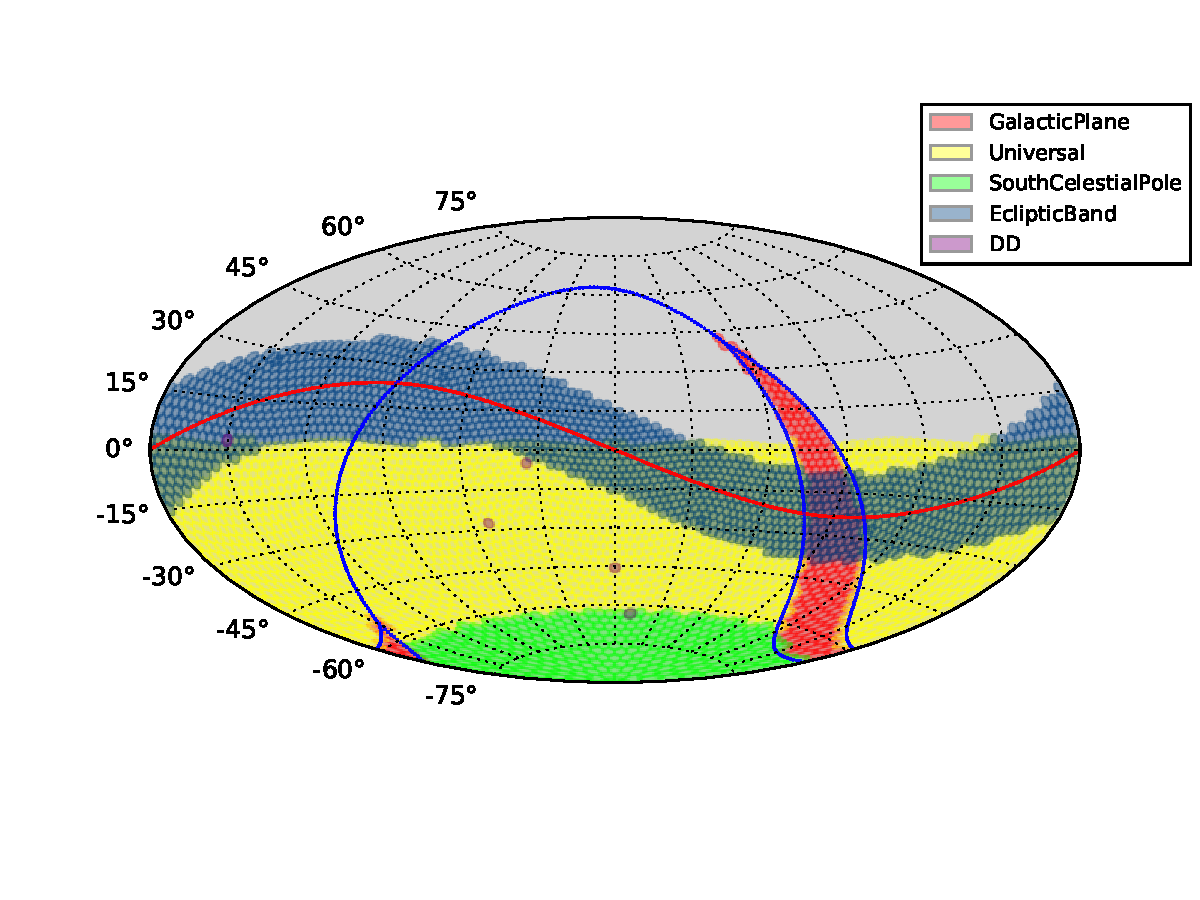
\includegraphics[width=0.45\textwidth]{figures/astro_lsst_01_1015_proposal_footprint}
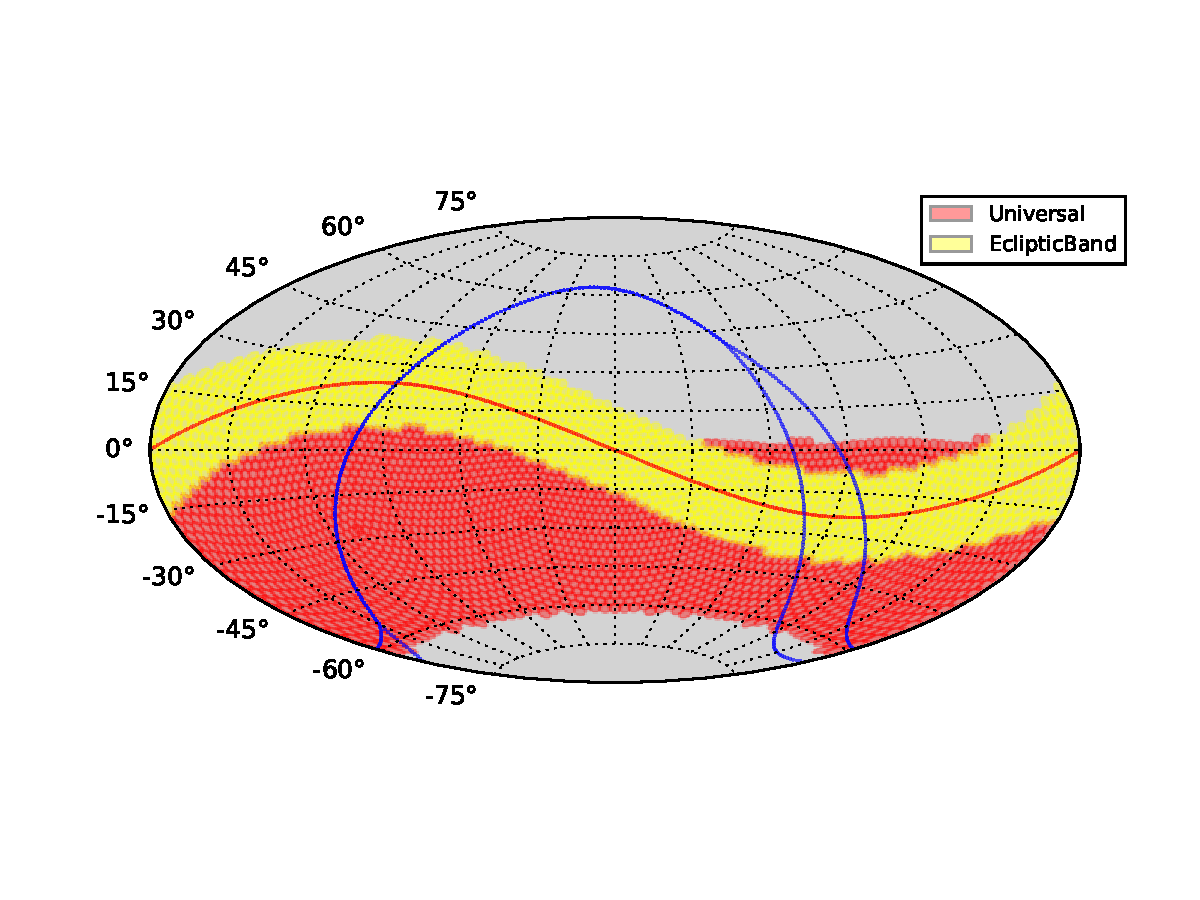
\includegraphics[width=0.45\textwidth]{figures/astro_lsst_01_1017_proposal_footprint}
\caption{The footprints of the proposals, including the Ecliptic Band proposal, used in the NEO-optimized simulated surveys astro\_lsst\_01\_1015 (left) and astro\_lsst\_01\_1017 (right). The astro\_lsst\_01\_1017 survey only includes two proposals.
\label{fig:neo_footprints}}
\end{figure}

\subsection{Completeness analysis results}

summarize completeness changes 

first for just pairs / triplets / quads

then for NEO-optimized runs, using pairs

\begin{enumerate}
\item baseline (minion1016) to more observations in NES
\item adding two years to astrolsst011016
\item extending MOPS window to 30 days, at SNR=5
\item adding longer exposures throughout the ecliptic (astrolsst011015/astrolsst1017)
\item making DM find objects with trailing loss, not detection losses
\item extending SNR limit to 4 instead of 5
\end{enumerate}

\subsection{Comparison with external completeness analysis}

The leading systematic effects in completeness estimates are: 
\begin{enumerate}
\item NEO vs. PHA difference (the completeness is about $\sim$10\% higher for PHAs than for NEOs) 
\item Different sample definitions: $H<22$ vs. $D>140$m (as shown by \citep{GMS2016}, completeness increases by $\sim$5\% when $H$-based criterion is used) 
\item Variations of ``discovery window'' (e.g., X visit pairs in N nights: changing N from 15 to 30 with X=3 increases
          completeness by 3\%; changing X from 3 to 4 with N=15 decreases completeness by 6\%). 
\item Sensitivity to details in sky coverage and cadence (e.g. nightly pairs of visits vs. quads of visits;
          requiring quads instead of pairs of visits decreases completeness by 30\% using baseline cadence; 
          about half of that loss can be recovered using cadence simulations that request four visits per night) 
\end{enumerate}          
    
\subsection{Remaining uncertainties in completeness estimates}

Common to all, really.          

\begin{enumerate}
\item Orbital parameter distribution for the simulated asteroid population (e.g. the Bottke model
             vs. the Granvik model); varying populations contribute completeness uncertainty of about a few percent) 
\\item Uncertainties when predicting effective image depth (system throughput, variation of the detection efficiency
          with the signal-to-noise ratio, treatment of trailing losses); for a survey that has a completeness above 60\%, 
          each additional 0.1 magnitude of depth for a given survey cadence increases the completeness by another 1\%.
\item Uncertainties when predicting asteroid's apparent flux (albedo distribution, phase effects, photometric variability 
          due to non-spherical shapes, color distributions); assuming an uncertainty of 0.2 mag in the effective 
          limiting magnitude, the corresponding  systematic uncertainty in completeness is about 2\%.)
\item The slope of the asteroid size distribution (current measurement uncertainty of this parameter 
          corresponds to a systematic uncertainty in completeness of about 2\%.)
\item The impact of known objects: assuming that 43\% objects would be discovered by the start of
          LSST survey, \cite{GMS2016} boosted the final PHA completeness for LSST baseline survey by 11\%. 
\end{enumerate} 

Given these systematic effects, a comparison of different simulation results (both for the same system,
and those of different systems, especially systems operating at different wavelengths) has to be undertaken
with due care. It is unlikely that a meaningful quantitative comparison can be pushed beyond a level
of a few percent (and perhaps as much as 10\%). In practice, the completeness of a given operating survey
is best estimated using the object re-discovery rate. 

